\documentclass[11pt,a4paper]{article}

\usepackage{amsmath, amssymb}
\usepackage{graphicx}
\usepackage{hyperref}
\usepackage{geometry}
\usepackage{mathtools}
\usepackage{mathrsfs}
\usepackage{tikz}
\usepackage{amsthm}
\usepackage[ruled,noend]{algorithm2e}
\SetKwFor{ForEach}{For all}{do}{}
\SetKwFor{For}{For}{do}{}
\SetKwIF{Si}{SinonSi}{Sinon}{Si}{alors}{Sinon si}{Sinon}{}
\SetKwInput{Input}{Input}
\SetKwInput{Output}{Output}
\SetKwProg{myproc}{Procedure}{:}{}
\SetKw{Return}{Return}
\SetKwComment{tcc}{(*}{*)}
\SetKwFor{Tq}{While}{Do}{}
\SetKwRepeat{Repeter}{répéter}{jusqu’à}
\geometry{margin=2.5cm}
\title{Computation of Minimum Absent Words and Minimum $p$-Absent Words}
\author{Jean Toulzac, Aloys Paupe}
\date{}

\begin{document}

\newtheorem{theoreme}{Theorem}
\newtheorem{lemme}{Lemma}
\newtheorem*{cor}{Corollary}
\newtheorem{prop}{Proposition}
\theoremstyle{definition}
\newtheorem{defin}{Definition}
\newtheorem*{ex}{Exemple}
\newtheorem*{cex}{Counter-exemple}
\theoremstyle{remark}
\newtheorem*{rem}{Remark}
\newtheorem{exer}{Exercise}
\newtheorem{qu}{Question}[exer]
\maketitle

\begin{abstract}
One of the most significant breakthroughs in computational biology has been the discovery 
of CRISPR (Clustered Regularly Interspaced Short Palindromic Repeats). This system functions as an adaptive immunity mechanism,
employed by bacteria to defend against bacterial viruses (phages) and predatory plasmids.
It shares a notable analogy with computer antiviruses – every DNA molecule entering a bacterium is compared with an “internal database”
of known “malicious code,” and if a match is found, the molecule is destroyed, similarly to
how computer antivirus eliminates malicious code before execution.
However, to evade detection, viruses and plasmids have developed sophisticated anti-defense systems
and evolved to avoid certain patterns, such as words stored in their “internal databases”. 
All these mechanisms are of a great interest for the biologists, and new mechanisms might be discovered 
from the study of those words that plasmids avoid.
The project’s goal is to identify minimal words absent in a major plasmid dataset, to
provide insights into words potentially targeted by CRISPR-Cas across diverse bacteria.

In this paper, we present naive algorithms for computing MAWs and $p$MAWs, 
as well as an improved approach based on properties of $k$-mers to reduce the search space.
\end{abstract}

\section{Minimum Absent Words (MAW)}
\subsection{Definition}
\begin{itemize}
    \item \textbf{Absent word: } Let $x$ and $s$ be two strings on the alphabet $\Sigma$. We say that $x$ is an
    \textit{absent word} of $S$ if neither $x$ nor its reverse complement occur as a substring of $S$.
    \item \textbf{Minimal absent word: } Let $x$ be a string of length $|x| > 1$ and $S$ be a string. We say
    that $x$ is a minimal absent word of $S$ if both the following conditions hold:
    \begin{enumerate}
        \item $x$ is an absent word of $S$;
        \item for every substring $w$ of $x$ such that $|w| < |x|$, it holds that $w$ or its reverse
        complement is a substring of at least one element of $S$.
    \end{enumerate}
  	\item We denote by $\mathcal{K}_S(k)$ the number of distinct $k$-mers in $S$
\end{itemize}

\subsection{Goal}
The goal is to implement one (or more) approaches to enumerate all
minimal absent words in each DNA sequence $s$ $\in$ $S$ that are shorter than a user-specified
length $k_{max}$, where $S$ denotes a user-provided set of input sequences.
\subsubsection{Implementation}
All implementation has been done in Python 3.12.3 on a laptop PC with one core of 11th Gen Intel(R) Core(TM) i5-1155G7 CPU at 2.50GHz and 8Gb of memory under 64-bit Linux. All testing was done on \texttt{all\_ebi\_plasmids.fa.xz} containing the EBI plasmid database
\subsection{Naive Algorithm}
We do not implement a purely naive algorithm; instead, we introduce a slight optimization.
Our approach is based on the following property: if all $k$-mers of a word $S$ are known, then any MAW of length $k+1$ must be of the form
\[
\alpha \omega \quad \text{or} \quad \omega \alpha,
\]
where:
\begin{itemize}
    \item $\omega$ is a $k$-mer occurring in $S$,
    \item $\alpha \in \Sigma$.
\end{itemize}
The generated candidate is then tested for occurrence in $S$; if it does not occur, it is considered a MAW.

Thus, rather than generating all possible words of length $k+1$,
we restrict candidate generation to extensions of existing $k$-mers by a single character from the alphabet, either on the left or on the right, which gets us the following algorithm:

\begin{algorithm}[H]
	\caption{Naive algorithm\label{algonaif}}
	\Input{A string $S$, an integer \texttt{k\_max}}
	\Output{The list of minimal absent words in $S$ of length up to \texttt{k\_max}}
	\tcc{\texttt{k\_mers}$(S,k)$ returns the set of $k$-mers of $S$}
	\texttt{res}$\gets\{\}$\\
	\For{$1<k<\texttt{k\_max}$}{
		\texttt{k\_mers\_set}$\gets$\texttt{k\_mers}$(S,k)$\\
		\ForEach{$x\in\texttt{k\_mers\_set}$}{
		\ForEach{$\alpha\in\Sigma$}{
			\If{$\alpha\cdot x\notin S$ and $\alpha\cdot x[:-1]\in\texttt{k\_mers\_set}$}{
				\texttt{res}$\gets\texttt{res}\cup\{\alpha\cdot x\}$
			}
		}
		}
	}
\end{algorithm}
\subsubsection{Correctness}
\paragraph{Every generated word is a minimal absent word}
If $w$ is outputed by our algorithm, it means there is a $k$-mer $x$ and $\alpha\in\Sigma$ such that $w=\alpha\cdot x$, $\alpha\cdot x\notin S$ and $\alpha\cdot x[:-1]$ is a $k$-mer, in which case since $x$ is a k-mer, all subwords  of $w$ are $k$-mers and $w$ is not a subword of $S$ therefore it is a minimal absent word.
\paragraph{Every minimal absent word is generated}
If $w$ is a minimal absent word, there exist a $k$-mer $x$ such that $x=w[1:]$ therefore since we look at every $k$-mer, the algorithm will study $x$ and since $w[0]\in\Sigma$, it will check that $w[0]\cdot x=w$ is not in $S$ (which is true since $w$ is an absent word) and that $w[0]\cdot[x:-1]$ is a $k$-mer, which is true since it is a subword of $w$ which is a minimal absent word, which means that $w$ will be outputed by the algorithm.
\subsubsection{Complexity}
\paragraph{Time complexity}
For every $k$ lower than $k_{max}$:
\begin{itemize}
	\item We build a set of $k$-mers, which is done with complexity $O(|S|)$
	\item For every $k$-mer, and every $\alpha\in\Sigma$, we check if words are in $S$ and in the set of $k$-mers, which is done respectively in average time complexity $O(|S|)$ and $O(\mathcal{K}_S(k))$
\end{itemize}
Thus the total average time complexity is $O\left(\sum\limits_{k=1}^{k_{max}-1}\times \left(|S|+\mathcal{K}_S(k)\times2\left(|S|+\mathcal{K}_S(k)\right)\right)\right)$. See the computation times in practice below.
\begin{table}[h!]
	\centering
	\begin{tabular}{|c|c|c|c|}
		\hline
		Value of $k_{max}$&1&2&3\\
		\hline
		Computation time (s) &647.6&1024.7&1560.8\\
		\hline
	\end{tabular}
	\caption{Computation times of algorithm $\ref{algonaif}$}
\end{table}
We didn't test the algorithm for $k_{max}$ greater than 3 beacause it is already exceedingly long for the lowest values.
\paragraph{Space complexity}
For every $k$ lower than $k_{max}$, we need to store the set of $k$-mers in $S$. We simply use an array and not a particular data structure, which means it has a space complexity of $O(k\times\mathcal{K}_S(k))$ and since we can get rid of the sets when $k$ increases, the total space complexity is of $O(k_{max}\times\mathcal{K}_S(k_{max}))$
\subsection{Our Idea}
Looking closer at minimal absent words, we realized that if $w$ is a minimal absent word of length $k$ for a read $S$, with $w_s=w[1:]$ and $w_p=w[:-1]$, $w_s$ and $w_p$ are both $(k-1)$-mers of $S$ but never appear "together" (meaning with $(k-2)$ common letters) since in that case $w$ would be a $k$-mer of $S$. This means that the first letter of $w_p$ and thus of $w$ can never appear before $w_s$ in $S$; and more precisely, we have:
\begin{prop}
	If $w$ is a word of length $k$, and $w_s$ and $w_p$ are define as above, we have :
	\begin{align*}
		w\text{ is a minimal absent word of }S \Leftrightarrow& w_p \text{ and } w_s\text{ are }(k-1)\text{-mers of }S
		\text{ and the first}\\&\text{letter of }w_p\text{ never appears before }w_s
	\end{align*}
	\label{prop1}
\end{prop}
\begin{proof}
	\indent If $w$ is a minimal absent word of $S$, then by definition, $w_p$ and $w_s$ are $(k-1)$-mers of $S$ and the first letter of $w_p$ never appears before $w_s$ because if it did, then $w_p[0]\cdot w_s=w$ would appear in $S$ which is absurd.\\
	\indent If $w_p$ and $w_s$ are two $(k-1)$-mers of $S$ such that $w_p[1:]=w_s[:-1]$ and the first letter of $w_p$ never appears before $w_s$, then we define $w=w_p[0]\cdot w_s$. Every subword of $w$ is either $w_p$, $w_s$ or a subword of those two, and thus is a subword of $S$, and $w$ is not a $k$-mer of $S$ because if it was, there would be an occurence of $w[0]=w_p[0]$ before $w_s=w[1:]$ which is absurd.
\end{proof}
This results gives us an easier way to look for minimal absent words. We simply have to look at every $(k-1)$-mer (which will have the role of $w_s$), and look for letters $l$ appearing before its longest proper prefix ($l\cdot w_s[:-1]$ will have the role of $w_p$) but not before it. From this idea, we write the following algorithm:\\
\begin{algorithm}[H]
	\caption{Efficient MAW computation\label{algo1}}
	\Input{A string $S$, an integer \texttt{k\_max}}
	\Output{The set of minimal absent words of $S$ of size smaller than \texttt{k\_max}}
	\tcc{ \texttt{k\_mers}$(string,k)$ returns a dictionary associating every $k$-mer of $string$ to the set of letters occuring before it in $string$}
	\texttt{res}$\gets\{\}$\\
	\For{$1<$\texttt{k}$\leq$\texttt{k\_max}}{
		\texttt{w\_s\_set}$\gets$\texttt{k\_mers}$(S,k)$\\
		\texttt{w\_p\_set}$\gets$\texttt{k\_mers}$(S,k-1)$\\
		\ForEach{\texttt{w\_s}$\in$\texttt{w\_s\_set}}{
		\texttt{w\_p}$\gets$\texttt{w\_s}$[:-1]$\\
		\texttt{letters\_candidates}$\gets$\texttt{w\_p\_set}$(\texttt{w\_p})\backslash$\texttt{w\_s\_set}$(\texttt{w\_s})$\\
		\texttt{res}$\gets$\texttt{res}$\cup\{\texttt{l}\cdot\texttt{w\_s}\mid\texttt{l}\in\texttt{letters\_candidates}\}$
		}
	}
	\Return{$\{\texttt{canonical}(w)\mid w\in\texttt{res}, \texttt{canonical}(w)\in\texttt{res}\}$}
\end{algorithm}
And we have:\\
\begin{algorithm}[H]
	\caption{\texttt{k\_mers}}
	\Input{A string $S$, an integer $k$}
	\Output{A dictionary association to every $k$-mer of $S$ the set of letters occuring before it}
	\texttt{dic}$\gets\{\}$\\
	$i\gets 0$\\
	$l\gets|S|$\\
	\While{$i+k<l$}{
		$seq\gets S[i:i+k+1]$\\
		\texttt{dic}$[seq]\gets\texttt{dic}[seq]\cup\{S[i-1]\}$\\
		$i\gets i+1$
	}
	\Return{\texttt{dic}}
\end{algorithm}
\subsubsection{Correctness}
\paragraph{Every generated word is a minimal absent word}
If $w$ is outputed by our algorithm, it means there is an element $w_s$ of \texttt{w\_s\_set} such that the first letter of $w$ appears before $w_s[:-1]$ but not $w_s$, therefore, with $w_p=w[0]\cdot w_s[:-1]$, we have that $w_p=w[:-1]$, $w_s=w[1:]$, and the first letter of $w_p$ never appears before $w_s$, thus from proposition $\ref{prop1}$, $w$ is a minimal absent word.
\paragraph{Every minimal absent word is generated}
If $w$ is a minimal absent word, from proposition $\ref{prop1}$, there exist two subwords of $S$, $w_p$ and $w_s$ such that $w_p=w[:-1]$ and $w_s=w[1:]$, and the first letter of $w_p$ never appears before $w_s$. Therefore, the set of letters preceding $w_s$ will not contain $w[0]$ whereas that of $w_p[1:]$ will. In addition, $w_p[1:]=w_s[:-1]$ and since $w_s$ is a subword of $S$, it will be in \texttt{w\_s\_set} which means that it will get looked at, and we will have \texttt{w\_p}$=$\texttt{w\_s}$[:-1]$ thus $w[0]$ will be in the candidate letters, and thus $w[0]\cdot w_s=w$ will be outputed
\subsubsection{Complexity}
\paragraph{Time complexity}
There are two parts to the algorithm:
\paragraph{Construction of the dictionaries}
For every $k$-mer, we compute a union of sets which has complexity $O(|\Sigma|)$, and this is done for every $k$-mer therefore the construction of a dictionary has an average time complexity of $O(|\Sigma|\times |S|)$ since dictionary operations have average complexity $O(1)$.
\paragraph{Main algorithm}
\begin{itemize}
	\item For every read $S$, we start by calculating every dictionary up to $k_{max}$, which is done with average time complexity $O(k_{max}\times|\Sigma|\times|S|)$.
	\item Then, for every $k$-mer, we calculate the difference between its preceding letters and those of its greatest proper prefix, which is done with complexity $O(|\Sigma|)$, and since this is done for every $k$-mer for $k$ up to $k_{max}$, it is done with complexity $O\left(|\Sigma|\times\sum\limits_{k=1}^{k_{max}}\mathcal{K}_S(k)\right)$
\end{itemize}
It is a bit hard to estimate the amount of distinct $k$-mers in a read, but in practice, the operation taking the most time was the construction of the dictionaries. See the experimental computation times below.
\begin{table}[h!]
	\centering
	\begin{tabular}{|c|c|c|c|c|c|c|c|}
		\hline Value of $k_{max}$&1&2&3&4&5&8&10\\
		\hline Computation time (s)&12.7&114.9&131.5&198.8&261.2&635.3&1944.8\\
		\hline
	\end{tabular}
	\caption{Computation times of algorithm $\ref{algo1}$}
\end{table}
\paragraph{Space complexity}
Similarly to the naive approach, we need to store the $k$-mers but this time we need two sets at the same time (the $k$-mers and the $(k-1)$-mers) which means our space complexity is of $O(k_{max}\times\mathcal{K}_S(k_{max})+(k_{max}-1)\times\mathcal{K}_S(k_{max}-1))$
\subsection{Improvement of complexity}
Although a lot better than the naive method, our algorithm is still very slow. One reason for this is that calculating the $k$-mers takes a lot of time, and we have to do it $k_{max}$ times per read; however, it's easy to see that while calculating the $k$-mers, we also get information on the smaller $p$-mers and the letters occuring before them, since the letter appearing before the $k$-mer at position $i$ is the same as the one appearing before the $(k-1)$-mer at position $i$: it's the letter at position $i-1$. This gave us the idea of using another data structure than the standard python dictionary: the radix tree.
\subsubsection{What is a radix tree}
\begin{defin}
	A radix tree is a tree where nodes with a single child are fused with it
\end{defin}
\begin{figure}[h!]
	\centering
	\begin{minipage}{0.48\linewidth}
		\centering
	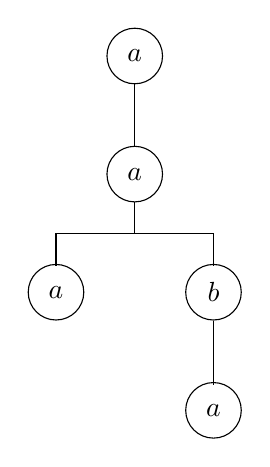
\begin{tikzpicture}
		\node at (0,1.5) {$a$};
		\node at (0,0) {$a$};
		\node at (-1,-1.5) {$a$};
		\node at (1,-1.5) {$b$};
		\node at (1,-3) {$a$};
		\draw (0,0) circle (10px);
		\draw (0,1.5) circle (10px);
		\draw (-1,-1.5) circle (10px);
		\draw (1,-1.5) circle (10px);
		\draw (1,-3) circle (10px);
		\draw (0,10px) -- (0,32.9px);
		\draw (0,-10px) -- (0,-0.75) -- (-1,-0.75) -- (-1,-32.9px);
		\draw (0,-10px) -- (0,-0.75) -- (1,-0.75) -- (1,-32.9px);
		\draw (1,-52.9px) -- (1,-75.8px);
	\end{tikzpicture}
	\caption{Example of a tree}
	\end{minipage}
	\begin{minipage}{0.48\linewidth}
		\centering
	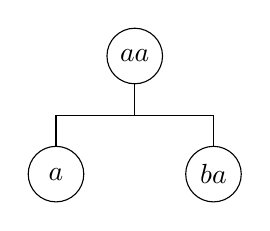
\begin{tikzpicture}
		\node at (0,0) {$aa$};
		\node at (-1,-1.5) {$a$};
		\node at (1,-1.5) {$ba$};
		\draw (0,0) circle (10px);
		\draw (-1,-1.5) circle (10px);
		\draw (1,-1.5) circle (10px);
		\draw (0,-10px) -- (0,-0.75) -- (-1,-0.75) -- (-1,-32.9px);
		\draw (0,-10px) -- (0,-0.75) -- (1,-0.75) -- (1,-32.9px);
	\end{tikzpicture}
	\caption{Corresponding radix tree}
	\end{minipage}
\end{figure}
\subsubsection{Why use radix trees}
By using a tree to store $k$-mers, when going down the tree to update $k-mers$ we can update the preceding letters for $p$-mers where $p$ is smaller than $k$. This way, by simply doing a depth-first-search of the tree, we will obtain all the information we want.
\subsubsection{Algorithm}
We use the implementation of radix trees from \cite{Charles2013} in which we modify the insert operation so that every visited node gets its preceding letters updated. Now, we first need to build the tree; before doing a depth-first search on it.\\
\begin{algorithm}[H]
	\caption{Construction of the tree}
	\Input{A string $S$, an integer $k_{max}$}
	\Output{A radix tree $t$ such that the node reach after reading $x$ contains the letters preceding $x$ in $S$}
	\tcc{\texttt{t.insert}$(k,d)$ inserts the node of key $k$ with data $d$ in tree $t$}
	$t\gets \texttt{RadixTree}()$\\
	$i\gets 0$\\
	$l\gets|S|$\\
	\While{$i+k_{max}<l$}{
		$t.\texttt{insert}(S[i:i+k],l[i-1])$
	}
	\While{$i<l$}{
		$t.\texttt{insert}(S[i:],l[i-1])$
	}
\end{algorithm}
\begin{algorithm}[H]
	\caption{Depth-First-Search}
	\Input{A radix tree $t$, an integer $k_{max}$, a list of nodes $l$}
	\Output{List of minimal absent words of length $k\leq k_{max}$}
	\texttt{res}$\gets$ list of size $k_{max}$ of empty sets\\
	\texttt{current\_node}$\gets t$\\
	\If{\texttt{current\_node} is not a leaf}{
		\ForEach{child $c$ of \texttt{current\_node}}{
			\texttt{temp}$\gets Depth-First-Search(c,k_{max}-\texttt{current\_node}.length,l\cup\{\texttt{current\_node}\})$\\
			\texttt{res}$\gets\texttt{res}+\texttt{temp}$
		}
	}
	\Else{
	$w\gets \varepsilon$\\
	\For{$1<i<|l|$}{
		$w\gets w\cdot l[i].name$\\
		\texttt{letters\_candidates}$\gets l[i-1].data\backslash l[i].data$\\
		\ForEach{$s\in\texttt{letters\_candidates}$}{
			\texttt{res}$[i]\gets\texttt{res}[i]\cup\{s\cdot w[:i]\}$
		}
	}}
	\Return{\texttt{res}}
\end{algorithm}
\subsubsection{Correctness}
\paragraph{The construction of the tree is correct}
\begin{itemize}
	\item If we insert a $k_{max}$-mer $u$ with preceding letter $l$, $l$ is also a preceeding letter for all the prefixes of $u$ so adding it as a preceeding letter to all visited nodes is correct.
	\item If a $k$-mer $u$ has a preceeding letter $l$, if it isn't at the very end of $S$, there also is a $k_{max}$-mer with $u$ as a prefix which has $l$ as a preceeding letter so it will get added, and if it is at the very end of $S$, the second loop takes care of it.
\end{itemize}
\paragraph{All generated words are minimal absent words}
If $x$ is outputed by the algorithm, it means there was a letter $s$ and an integer $i$ such that $x=s\cdot w[:i]$ was generated, with $w$ a read in the radix tree. Since $w$ is a read in the radix tree, it is a subword of $S$ therefore so is $w[:i]$, and since the tree is correct, similarly to the proof of correctness of the previous algorithm, we have a minimal absent word.
\paragraph{All minimal absent words are generated}
If $w$ is a minimal absent word, $w_s=w[1:]$ is a subword of $S$ and therefore can be found in the radix tree and gives its preceeding letters, as well as $w_s[:-1]$ which means that, similarly to the proof of correctness of the previous algorithm, $w$ will be produced.
\subsubsection{Complexity}
\paragraph{Time complexity}
There are two parts to the algorithm:
\paragraph{Construction of the tree}
Every insertion has average complexity $O(k_{max})$ thus the construction of the whole tree has average complexity $O(k_{max}\times|S|)$
\paragraph{Exploration of the tree}
A depth-first-search of the tree is done in worst case in $O(k_{max}\times \mathcal{K}_S(k_{max}))$ since it is the most nodes there can be in a tree, and every leaf explored leads to $O(k_{max})$ operations which the total time complexity is in worst case $O((k_{max}-1)\times(\mathcal{K}_S(k_{max}))+k_{max}\times\mathcal{K}_S(k_{max}))$. It should therefore be faster than our previous algorithm, however in practice, it is very slow, even slower than the naive algorithm, taking 5031 seconds simply for $k_{max}=1$. This may be because of the implementation of radix trees, and because we didn't have enough time to optimize the operations.
\paragraph{Space complexity}
the only thing to store is the radix tree containing the preceding letters, which means it takes space $O(|\Sigma|\times k_{max}\times \mathcal{K}_S(k_{max}))$ in the worst case.
\subsection{Possible improvements}
There are different avenues of improvement :
\begin{itemize}
	\item Using more optimized variants of the radix tree, such as the adaptative radix tree which changes node size based on the number of children, or the k-compact canonical trees which do not store complete subtrees but simply indicate it on the corresponding root.
	\item Considering the strong correlation between adjacent $k$-mers, it seems likely that there is no need to look at all of them, but we have not found a way to theorize it and take advantage of it.
\end{itemize}
\section{Minimum $p$-Absent Words ($p$MAW)}
\subsection{Definition}
\begin{itemize}
    \item \textbf{Minimum $p$-Absent Words: } Let $x$ be a string of length $|x| > 1$ and $S$ be a set of strings.
    We say that $x$ is a minimal $p$-absent word of $S$ if both the following
    conditions hold:
    \begin{enumerate}
        \item $x$ is an absent word of $S$ for at least $p · |S|$ sequences $s \in S$;
        \item for every substring $w$ of $x$ such that $|w| < |x|$, it holds that $w$ is not a $p$-absent
        word of $S$.
    \end{enumerate}
\end{itemize}

\subsection{Goal}
The goal is to implement one (or more) approaches to enumerate all
minimal $p$-absent words in each DNA sequence $s$ $\in$ $S$ that are shorter than a user-specified
length $k_{max}$, where $S$ denotes a user-provided set of input sequences, considering we have already calculated all the minimal absent words.
\subsection{Implementation}
All implementation is done in the same circumstances as the first program.
\subsection{Naive Algorithm}
Similarly to the naive algorithm for minimal absent words, we know that every minimal $p$-absent words is an extenxion of a $k$-mer so we can look only at those.\\
\begin{algorithm}[H]
	\caption{Naive $p$-MAW algorithm\label{pmawnaif}}
	\Input{A sequence $\mathcal{S}$ of strings $S$, an integer $k_{max}$, a float $p\in[0,1]$}
	\Output{The set of minimal $p$-absent words of $\mathcal{S}$}
	$res\gets\{\}$\\
	$candidates\gets\{\}$\\
	$k\_mers\gets$ dictionary on $\mathcal{S}$ of sets of mers\\
	\ForEach{$k$-mer $x$}{
		\ForEach{$\alpha\in \Sigma$}{
		\If{$\alpha\cdot x$ is absent from at least $p\times|\mathcal{S}|$ reads}{
		$candidates\gets candidates\cup\{\alpha\cdot x\}$
		}
		}
	}
	\ForEach{$x\in candidates$}{
		\If{$x[1:]\notin candidates$ and $x[:-1]\notin candidates$}{
		$res\gets res\cup\{x\}$
		}
	}
	\Return{$res$}
\end{algorithm}
\subsubsection{Correctness}
\paragraph{Every generated word is a minimal $p$-absent word}
If $w$ is outputed by the algorithm, then there is a $\alpha\in\Sigma$ such that $w[0]=\alpha$, $w=\alpha\cdot x$, $w$ is absent from at least $p\times|\mathcal{S}|$ (is a $p$-absent word), and $x$ and $w[:-1]$ are not $p$-absent words. This means that no subword of $w$ is a $p$-absent word and since $w$ is one, it is a minimal $p$-absent word.
\paragraph{Every minimal $p$-absent word is generated} 
If $w$ is a minimal $p$-absent word, with $w_s=w[1:]$, $w_s$ is a $k$-mer of a read, which means it is in the set of all kmers and $w[0]\cdot w_s$ is absent from at least $p\times|\mathcal{S}|$ reads therefore $w$ is added to $candidates$. Later, $w$ will get studied as an element of $candidates$, and since it is a minimal $p$-absent word, $w[1:]$ and $w[:-1]$ are not and thus $x$ is accepted as a minimal $p$-absent word.
\subsubsection{Complexity}
\paragraph{Time complexity} There are three steps to the algorithm:
\paragraph{Construction of the set of $k$-mers}
We won't get into details due to it being very similar to previous algorithms, but it is done in $O\left(k_{max}\times\sum\limits_{S\in\mathcal{S}}|S|\right)$
\paragraph{Selection of candidates}
Checking if $\alpha\cdot x$ is in at least $p\times |\mathcal{S}|$ reads is done with time complexity $O\left(\sum\limits_{S\in\mathcal{S}}|S|\right)$ thus the selection of candidates is done with complexity $O\left(\mathcal{K}_\mathcal{S}\times |\Sigma|\times \sum\limits_{S\in\mathcal{S}}|S|\right)$
\paragraph{Selection among candidates}
Checking whether $x[1:]$ and $x[:-1]$ are in $candidates$ is done with complexity $O(|candidates|)$ thus this step is done with complexity $O\left(|candidates|^2\right)$. It is a bit hard to estimate the amount of candidates, but it is in worst case $\mathcal{K}_\mathcal{S}$. We can see the computation times in practice below.
\paragraph{Space complexity}
This algorithm is rather heavy in space complexity. For our quick implementation, we stored $k$-mers for each read as well as a set of every $k$-mer (which could be done more efficiently by storing with every $k$-mer the set of reads in which it appears) which has a total space complexity of $O(2\times\mathcal{K}_\mathcal{S})$ and storing the candidates takes up another $O(|candidates|)$, which is $O(\mathcal{K}_\mathcal{S})$ in the worst case.
\begin{table}[h!]
	\centering
	\begin{tabular}{|c|c|c|c|c|}
		\hline
		Values of $k_{max}$&2&3&4&5\\
		\hline
		Computation time (s)&374.8&751.4&1230&1628\\
		\hline
	\end{tabular}
	\caption{Computation times of algorithm $\ref{pmawnaif}$ with $p=0.5$}
\end{table}
\subsection{Our Idea}
Once again, the naive algorithm is very slow, and most importantly, it does not take advantage of the already calculated minimal absent words. For our new algorithm, we take it into account with proposition $\ref{prop2}$
\begin{prop}
	If $w$ is a minimal $p$-absent word of sequence $\mathcal{S}$, there are words $u$, $v_1$ and $v_2$ such that $u$ is a minimal absent word for at least one read $S$ of $\mathcal{S}$ and $w=v_1\cdot u\cdot v_2$ \label{prop2}
\end{prop}
\begin{proof}
	There are two possibilities :
	\begin{enumerate}
		\item $w$ is a MAW for a read $S$ in which case with $u=w$ and $v=\varepsilon$ we have the property
		\item $w$ is not a MAW, in which case since $w$ is a $p$MAW, there is a read $S$ where $w$ is absent but since it isn't a MAW, either $w_s=w[1:]$ or $w_p=w[:-1]$ isn't a subword of $S$. Without loss of generality, let's assume $w_s$ is not a subword of $S$: we can iterate the reasoning on $w_s$ until we find a word whose every subword belongs to $S$, which will happen since $|w_s|<w$.
	\end{enumerate}
	Since every subword is chosen so as not to belong to $S$, the resulting word $u$ will be a MAW and thus $w$ will be written $v_1\cdot u \cdot v_2$ for some $v_1,v_2$.
\end{proof}
Using this, we will look for $p$MAW candidates only among MAWs and their extensions. 

\subsubsection{Algorithm}
\begin{algorithm}[H]
	\caption{Candidates}
	\Input{A sequence of string $\mathcal{S}$, an integer $k_{max}$, a float $p\in[0,1]$, a word $w$}
	\Output{The set of potential $p$MAW which extend from $w$}
	\tcc{Every $k$-mer has a bit $visited$ in order to avoid looking at the same $k$-mer twice}
	$w.visited\gets 1$\\
	\If{$|w|\leq k_{max}$ and $w$ is absent from at least $p\times|\mathcal{S}|$ reads}{
		\Return{$\{w\}$}
	}
	\If{$|w|\geq k_{max}$}{
		\Return{$\{\}$}
	}
	$candidates\gets\{\}$\\
	\ForEach{$\alpha\in\Sigma$}{
		$x\gets \alpha\cdot w$\\
		\If{$\neg x.visited$}{
			\If{$x$ is absent from at least $p\times|\mathcal{S}|$ reads}{
				$candidates\gets candidates\cup\{x\}$\\
				$x.visited\gets 1$
			}
			\Else{
				$candidates\gets candidates\cup Candidates(\mathcal{S},k_{max},p,x)$
			}
		}
		$x\gets w\cdot \alpha$\\
		\If{$\neg x.visited$}{
			\If{$x$ is absent from at least $p\times|\mathcal{S}|$ reads}{
				$candidates\gets candidates\cup\{x\}$\\
				$x.visited\gets 1$
			}
			\Else{
				$candidates\gets candidates\cup Candidates(\mathcal{S},k_{max},p,x)$
			}
		}
	}
	\Return{$candidates$}
\end{algorithm}
\begin{algorithm}
	\caption{Efficient $p$MAW computation\label{pmawsmart}}
	\Input{A sequence of reads $\mathcal{S}$, a dictionary of sets of MAWs $\mathcal{M}$ of length $|\mathcal{S}|$ , an integer $k_{max}$, a float $p\in[0,1]$}
	\Output{The set of all $p$-MAWs of $\mathcal{S}$}
	$res\gets\{\}$\\
	$candidates\gets\{\}$\\
	\ForEach{$w\in\mathcal{M}(S)$}{
		$candidates\gets candidates\cup Candidates(S,k_{max},p,w)$
	}
	\ForEach{$w\in candidates$}{
		$ispMAW\gets True$\\
		\ForEach{substring $x$ of $w$}{
			\If{$x\in candidates$}{
				$ispMAW\gets False$
			}
		}
		\If{$ispMAW$}{
			$res\gets res\cup\{w\}$
		}
	}
\end{algorithm}
\subsubsection{Correctness}
There are two parts to the algorithm:
\paragraph{Candidate selection is correct}
\begin{prop}
	All words outputed by $Candidates$ are $p$-absent words and all minimal $p$-absent words are outputed by $Candidates$ \label{prop3}
\end{prop}
\begin{proof}
	\begin{itemize}
		\item Let $x$ be a word outputed by $Candidates(\mathcal{S},k_{max},p,w)$, let's prove by induction over $|x|$ that all outputs are $p$-absent words:
		\begin{itemize}
			\item If $|x|=k_{max}$, $x$ can only be outputed if it is a $p$-absent word
			\item If $|x|<k_{max}$, then it had not been visited before, and either it is returned because it is a $p$-absent word, or we return $Candidates(\mathcal{S},k_{max},p,y)$ where $y$ is an extension of $x$, and thus of strictly greater length which means all its outputs are $p$-absent words by induction hypothesis
		\end{itemize} 
		Thus every word outputed by $Candidates$ is a $p$-absent word.
		\item Let $w$ be a minimal $p$-absent word. If it is a MAW, since it is $p$-absent and we call $Candidates$ on all MAWs, it is outputed by $Candidates$. If not, we know from proposition $\ref{prop2}$ that there exist $v_1,v_2$ two words and $u$ a MAW such that $w=v_1\cdot u\cdot v_2$, therefore $Candidates$ will be called on $u$, and it will extend $u$ until it finds a $p$-absent word. It cannot stop before $w$ since that would mean that $w$ has a subword that is $p$-absent, therefore it outputs $w$.
	\end{itemize}
\end{proof}
\paragraph{Every generated word is a minimal $p$-absent word}
Let $w$ be a word outputed by the algorithm. Let's assume that it is not a minimal $p$-absent word. Since it is a $p$-absent word from proposition $\ref{prop3}$, there is a proper subword $u$ of $w$ which is a minimal $p$-absent word and thus appears in $candidates$ which means there is a subword of $w$ in $candidates$ which is absurd, thus every generated word is a minimal $p$-absent word.
\paragraph{Every minimal $p$-absent word is generated}
Let $w$ be a minimal $p$-absent word. From proposition $\ref{prop3}$, $w$ appears in $candidates$, and since every element of $candidates$ is a $p$-absent word, no proper subword of $w$ appears in $candidates$ which means it is outputed.
\subsubsection{Complexity}
\paragraph{Time complexity}
There are two parts to the algorithm:
\paragraph{Candidate selection}
The number of extensions of a word is in $O(|\Sigma|^{k_{max}})$ and every extension is checked for membership in $O(|S|\times k_{max})$ which gives us a total complexity of $O(|S|\times k_{max}\times |\Sigma|^{k_{max}})$
\paragraph{Main algorithm}
We generate candidates from every MAW with complexity $O(|MAW|\times |S|\times k_{max})$ and for each candidate we check for membership in $O(|candidates|)$ for $O(k_{max}^2)$ subwords, which gives us a total complexity of $O(|MAW|\times |S| \times k_{max}+|candidates|^2\times(k_{max}^2))$. See below the computation times obtained in practice
\begin{table}
	\centering
	\begin{tabular}{|c|c|c|c|}
		\hline
		Value of $k_{max}$&3&4&5\\
		\hline
		Computation time (s)&609.9&1445.9&3384.7\\
		\hline
	\end{tabular}
	\caption{Computation time of algorithm $\ref{pmawsmart}$}
\end{table}
\paragraph{Space complexity}
We need to store every candidate and keep information on visited words for a worst-case space complexity of $O(k_{max}\times\mathcal{K}_\mathcal{S}(k_{max}+1))$ since we look at at most $O(\mathcal{K}_\mathcal{S}\times k_{max})$ different words
\section{Conclusion}
\subsection{Findings}
We have managed to construct 5 different algorithms, 3 for the generation of minimal absent words and 2 for the generation of minimal $p$-absent words:
\begin{enumerate}
	\item A naive algorithm generating MAWs by extending upon $k$-mers and checking their subwords
	\item An efficient algorithm generating MAWs using the property explained in proposition $\ref{prop1}$ by looking at letters appearing before the $k$-mers in the read
	\item An improvement of the previous algorithm which stores $k$-mers in a radix tree, allowing for a single look through the read and through the tree to give us all the data we need, although in practice, our implementation gave us even worse times than the naive algorithm
	\item A naive algorithm generating $p$MAWs by extending upon $k$-mers and checking their subwords
	\item An efficient algorithm taking into account the fact that every $p$MAW is an extension of a MAW, although once again, in practice our implementation is slower than the naive algorithm
\end{enumerate}
\subsection{Improvement}
There are multiple things we would like to improve on:
\begin{itemize}
	\item Since we lacked time, we didn't get to do as much testing as we would have wanted, particulary for the $p$MAWs where we only tested the algorithms with one value of $p$ which was $0.5$.
	\item It should be possible to optimize our algorithms, at least enough so that the "smart" algorithms are faster than the naive ones. Right now, all of our algorithms, especially for $p$-absent words, are very slow.
\end{itemize}
\begin{thebibliography}{1}
\bibitem{Charles2013}
	N.Jeudy,radix-tree, 2024, GitHub, \url{https://github.com/Nicola-31/radix-tree#readme}
\end{thebibliography}

\end{document}
